% Analítica Predictiva y Prescriptiva · TIC-60286 · Semana 6
% Árboles de regresión
% Compilar: pdflatex week-06.tex (dos veces)
%
% Plan de los 90 minutos
%   0–5    Dónde vamos y la parada 1: la encuesta por rangos, el ancla (láminas 2–3)
%   5–20   El paper: Mullainathan y Spiess (2017), con las cuatro preguntas y el puente (láminas 4–7)
%  20–65   La aplicación: las varas, el árbol leído en voz alta, el ejemplo a mano (los ocho puntos de venta
%          de juguete y la hoja real de diez puntos de venta), la profundidad 3, la tabla del líder con el error
%          sembrado, la pareada, el memorizador con la parada 2, los diez peores, las ventas base con
%          banda y el giro del arriendo (láminas 8–21)
%  65–70   Puente: el task 6 (lámina 22)
%  70–90   Cierre: el task 5 que trajeron (lámina 23)
%
% Las cifras salen de datasets/aperturas/cifras_week06.txt y, las derivadas (el ejemplo a mano, el MAE de
% entrenamiento del error sembrado, la hoja de n = 10, el giro), de input/cifras_derivadas_week06.txt.
% Las figuras las genera input/_figuras_week06.R; figures/arbol_regresion_residuos.pdf es la figura base
% del generador del estudio de aperturas (datasets/aperturas/figuras/).
% La tabla 1 del paper se verificó el 10 de octubre de 2026 contra el artículo (reproducido en las
% láminas de A. C. Cameron, 2019) y contra la tabla B.1 del apéndice en línea de los autores:
% R² en entrenamiento / en prueba: regresión 47.3 / 41.7; árbol ajustado por profundidad 39.6 / 34.5;
% LASSO 46.0 / 43.3; bosque 85.1 / 45.5; ensamble 80.4 / 45.9 (intervalos de prueba de cerca de ± 2 puntos).

\documentclass{beamer}
\input{../../_beamer/preambulo_app.tex}
\semana{6}{Árboles de regresión}

\begin{document}

%%=================================================
%% Primer slide
\begin{frame}
\titlepage
\end{frame}

%% ====================================================== 0. DÓNDE VAMOS (0–5)
\begin{frame}{Dónde vamos}
\begin{columns}[T]
\begin{column}{0.5\textwidth}
\textbf{La semana pasada:} un árbol que responde sí o no. Lo leyeron como política, lo examinaron en validación y lo aplicaron a los tres locales con asterisco. Su task 5 se discute hoy, en el cierre.

\medskip
\textbf{Hoy, la pieza 6 del expediente:} el mismo árbol, preguntando un número. Cuánto vende un local, con qué error en pesos, si le gana a la regla del sector, dónde falla, y las ventas base con banda que entran al VPN de la semana 7.
\end{column}
\begin{column}{0.5\textwidth}
\begin{block}{La sesión}
\begin{enumerate}
  \item El paper: árboles, bosques y regresión prediciendo el valor de viviendas (2017).
  \item El árbol de ventas, leído en voz alta y rehecho a mano.
  \item La tabla del líder en pesos, con un error sembrado.
  \item Los diez peores, las bandas y un giro.
  \item Cierre: el task 5.
\end{enumerate}
\end{block}
\end{column}
\end{columns}
\end{frame}

\begin{frame}{Antes de empezar}
\parada{encuesta por rangos}{¿Cuánto vende al mes un punto de venta de conveniencia de \textbf{80 m\textsuperscript{2} en zona de oficinas en Barranquilla}? Marquen un rango: menos de 80 / de 80 a 120 / de 120 a 160 / de 160 a 200 / más de 200 millones.}
\medskip
\small Guarden su rango. Al final de la aplicación lo comparamos con lo que dice el árbol para un local parecido (el local 1, de 95 m\textsuperscript{2}) y con lo que dice la regla del sector. La cifra que cada uno marcó es su ancla: vamos a ver cuánto pesa.
\end{frame}

\seccion{El paper: predecir el valor de una vivienda}
%% ====================================================== 1. EL PAPER (5–20)
\begin{frame}{Qué aporta el aprendizaje automático a la economía aplicada}{Mullainathan y Spiess (2017), \emph{Journal of Economic Perspectives}}
\small
\begin{columns}[T]
\begin{column}{0.5\textwidth}
\textbf{Qué investigaron.} Qué puede hacer el aprendizaje automático por la economía aplicada. Su respuesta: predecir. La econometría clásica estima parámetros ($\hat\beta$: cuánto cambia $y$ cuando cambia $x$); el aprendizaje automático produce $\hat y$ (qué valor toma $y$ en una unidad nueva) sin prometer nada sobre los parámetros.

\medskip
\textbf{El ejemplo.} Predecir el valor de una vivienda a partir de sus características: el problema del avaluador instantáneo, y el nuestro a otra escala.
\end{column}
\begin{column}{0.5\textwidth}
\begin{block}{La distinción que organiza el paper}
\begin{itemize}\itemsep3pt
  \item \textbf{Predicción ($\hat y$):} se juzga por el error en datos nuevos; vale cualquier método que acierte.
  \item \textbf{Estimación ($\hat\beta$):} se juzga por si el coeficiente es el efecto; exige supuestos.
  \item Un buen $\hat y$ no da un buen $\hat\beta$: las variables que elige el algoritmo no son ``las causas''.
\end{itemize}
\end{block}
\end{column}
\end{columns}
\end{frame}

\begin{frame}{Qué datos y cómo}
\footnotesize
\begin{columns}[T]
\begin{column}{0.5\textwidth}
\begin{itemize}\itemsep3pt
  \item \textbf{American Housing Survey 2011}, muestra metropolitana: viviendas ocupadas por su propietario y el valor que el propietario declara (en logaritmo).
  \item \textbf{150 características} de la vivienda y su entorno (habitaciones, área, antigüedad, región, ciudad o suburbio), más doce indicadores de datos faltantes.
  \item \textbf{10.000 unidades de entrenamiento} y \textbf{41.808 de prueba}, separadas antes de ajustar nada.
\end{itemize}
\end{column}
\begin{column}{0.5\textwidth}
\begin{itemize}\itemsep3pt
  \item Cinco métodos: \textbf{regresión lineal} con las 150 variables, \textbf{árbol de regresión} ajustado por profundidad, \textbf{LASSO}, \textbf{bosque aleatorio} y un \textbf{ensamble} de los anteriores.
  \item Los frenos (la profundidad del árbol, la penalización del LASSO) se eligen por validación cruzada de ocho pliegues \emph{dentro} del entrenamiento.
  \item Todos se juzgan por el $R^2$ en las 41.808 unidades de prueba, que ningún método vio.
\end{itemize}
\end{column}
\end{columns}
\smallskip
\importa{La arquitectura del curso: un lote para construir, otro para examinar, y los frenos elegidos sin mirar el examen.}
\end{frame}

\begin{frame}{Qué encontraron}{Tabla 1 del paper: $R^2$ en entrenamiento y en prueba}
\begin{columns}[T]
\begin{column}{0.54\textwidth}
{\scriptsize\setlength{\tabcolsep}{4pt}
\begin{tabular}{@{}lrr@{}}
\toprule
Método & Entrenamiento & Prueba \\
\midrule
Regresión lineal & 47.3\,\% & 41.7\,\% \\
Árbol de regresión & 39.6\,\% & 34.5\,\% \\
LASSO & 46.0\,\% & 43.3\,\% \\
Bosque aleatorio & \textbf{85.1\,\%} & 45.5\,\% \\
Ensamble & 80.4\,\% & \textbf{45.9\,\%} \\
\bottomrule
\end{tabular}}
\smallskip

{\scriptsize El árbol, con la profundidad elegida por validación cruzada. Margen de dos errores estándar en prueba: cerca de $\pm$ 2 puntos en todas las filas.}
\end{column}
\begin{column}{0.46\textwidth}
\footnotesize
\begin{itemize}\itemsep3pt
  \item \textbf{El árbol solo pierde} con la regresión fuera de muestra: 34.5 contra 41.7.
  \item \textbf{El bosque ``memoriza'' y aun así gana:} 85.1 en entrenamiento, 45.5 en prueba. La cifra de entrenamiento no dice nada; la de prueba, todo.
  \item \textbf{El ensamble gana por poco} (45.9): ningún método domina en todos los tramos de valor.
  \item \textbf{Las variables que elige LASSO cambian} de una submuestra a otra (figura 2 del paper) \textbf{sin que cambie la calidad de la predicción}.
\end{itemize}
\end{column}
\end{columns}
\end{frame}

\begin{frame}{Por qué importa para quien decide}
\small
\begin{block}{Tres lecciones}
\begin{enumerate}\itemsep3pt
  \item \textbf{Un pronóstico se juzga por su error fuera de muestra}, en la unidad de la decisión. El ajuste en entrenamiento es un espejismo: el bosque sacó 85 y valía 45.
  \item \textbf{El árbol solo es tosco; el bosque promedia y gana.} Por eso la consultora B es un bosque y el árbol es su vocero: el bosque decide, el árbol explica.
  \item \textbf{Las variables del árbol no son las causas.} Otra muestra, otras variables, la misma calidad. A la junta se le cuenta lo que aguanta, no la lista.
\end{enumerate}
\end{block}
\parada{el puente}{Latitud tiene el estudio de aperturas (480 puntos de venta con sus ventas y doce variables de antes de abrir) y tres locales en Barranquilla. Necesita lo mismo que el avaluador: un pronóstico con su error en pesos, medido en puntos de venta que el método no vio, y una vara que vencer.}
\end{frame}

\seccion{La aplicación: el árbol de ventas de Latitud}
%% ====================================================== 2. LA APLICACIÓN (20–65)
\begin{frame}{Las varas: la mediana y la regla del sector}
\begin{columns}[T]
\begin{column}{0.5\textwidth}
\small
\textbf{La vara ingenua:} la mediana del entrenamiento, 93.1 millones para todos. MAE 31.1 en validación.
\medskip

\textbf{La vara exigente:} la regla del sector, ventas $\approx$ 8 $\times$ arriendo. La cuenta que un gerente de expansión hace de memoria. MAE \textbf{22.4} ($\pm$ 3.7), RMSE 30.0.
\medskip

Para Barranquilla: local 1, $8 \times 16.5 = 132$; local 2, $8 \times 27 = 216$; local 3, $8 \times 8 = 64$.
\end{column}
\begin{column}{0.5\textwidth}
\importa{Un modelo aporta solo lo que le gana a la vara. La semana 4 lo dejó claro con las consultoras: A empató con la regla y B le ganó por 4.4 millones al mes por punto de venta. Hoy el árbol entra a la misma tabla.}
\medskip
\footnotesize La regla no es ingenua: en estos datos el arriendo ya resume la ciudad, la zona, el área y el tráfico. Por eso la primera pregunta del árbol va a ser el arriendo.
\end{column}
\end{columns}
\end{frame}

\begin{frame}{El árbol de ventas, leído en voz alta}
\begin{columns}[T]
\begin{column}{0.58\textwidth}
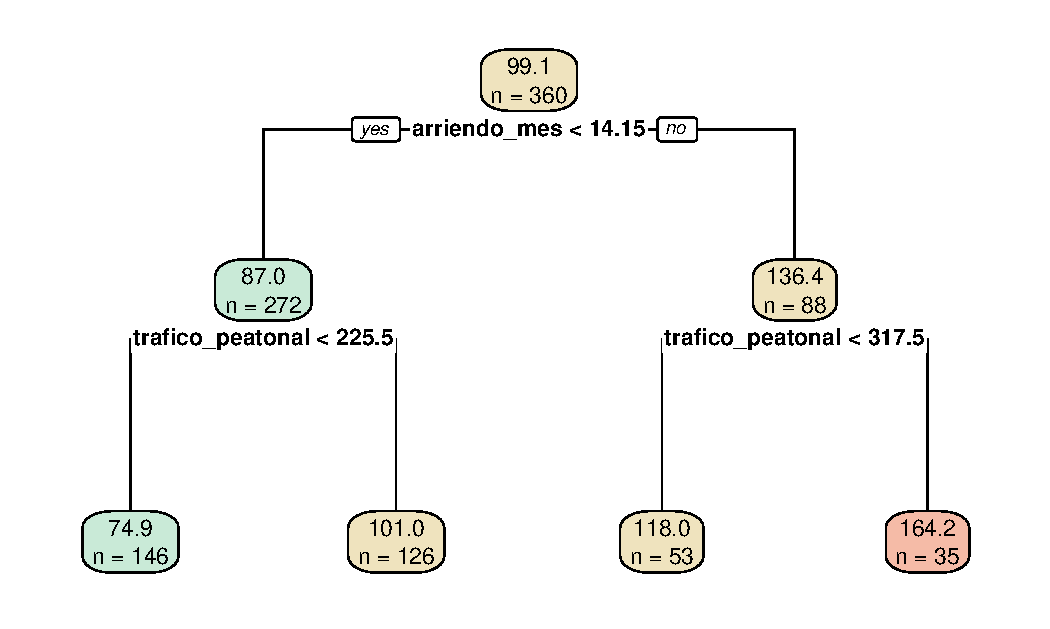
\includegraphics[width=\textwidth]{figures/arbol_regresion_2.pdf}
\end{column}
\begin{column}{0.42\textwidth}
\footnotesize
Profundidad 2, mínimo 10 por hoja, 360 puntos de venta, doce columnas de antes de abrir, método \texttt{anova}: cada hoja predice un promedio.
\medskip

\textbf{Arriendo bajo (menos de 14.15) y tráfico bajo:} 74.9 millones (n = 146).

\textbf{Arriendo bajo y tráfico de 226 o más:} 101.0 (n = 126).

\textbf{Arriendo alto y tráfico medio:} 118.0 (n = 53).

\textbf{Arriendo alto y tráfico de 318 o más:} 164.2 (n = 35).
\medskip

La raíz ya no es el tráfico: es el arriendo, que lo resume todo. ¿Coincide con su rango de la encuesta?
\end{column}
\end{columns}
\end{frame}

\begin{frame}{No creer, verificar: el promedio de una hoja a mano (I)}
\begin{center}
{\scriptsize
\begin{tabular}{@{}lrrrrrrrr@{}}
\toprule
Punto de venta & A & B & C & D & E & F & G & H \\
\midrule
Tráfico (personas por hora) & 90 & 110 & 130 & 150 & 190 & 260 & 340 & 520 \\
Ventas (millones al mes) & 50 & 56 & 66 & 68 & 96 & 104 & 130 & 150 \\
\bottomrule
\end{tabular}}
\end{center}
\begin{columns}[T]
\begin{column}{0.5\textwidth}
\footnotesize
\textbf{Corte en 170} (entre D y E): izquierda, promedio 60 y suma de cuadrados 216; derecha, promedio 120 y 1.832. Total \textbf{2.048}.
\smallskip

\textbf{Corte en 300} (entre F y G): izquierda 73.3 y 2.381; derecha 140 y 200. Total 2.581.
\smallskip

Sin corte: un solo promedio (90), 9.248.
\smallskip

\importa{El árbol ensaya los siete cortes y se queda con el que deja las hojas más apretadas. Una hoja es un promedio; un corte es una tabla de dos promedios.}
\end{column}
\begin{column}{0.5\textwidth}
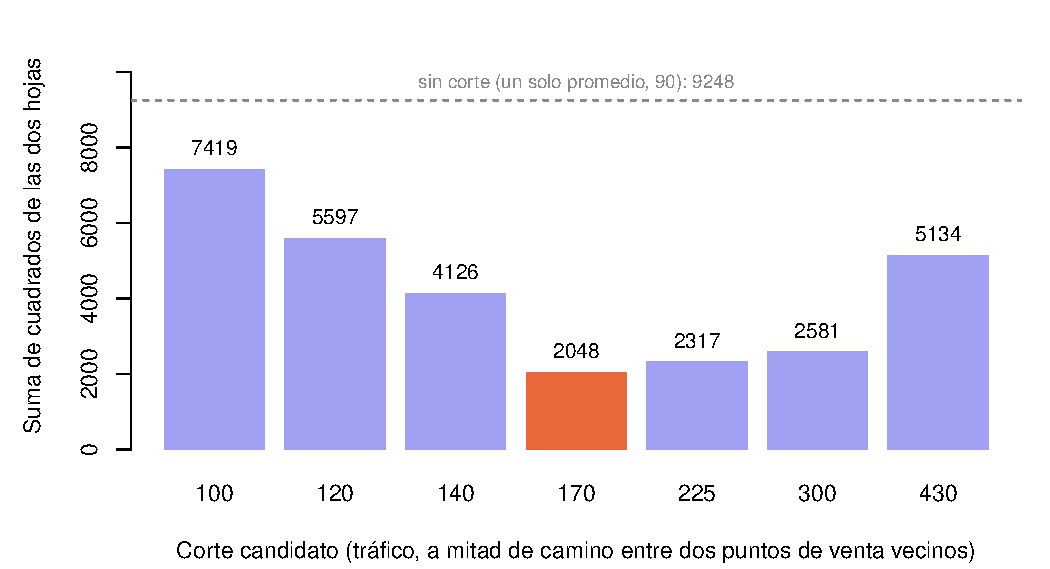
\includegraphics[width=\textwidth]{figures/cortes_juguete.pdf}
\end{column}
\end{columns}
\end{frame}

\begin{frame}{El promedio de una hoja a mano (II): una escalera, no una rampa}
\begin{center}
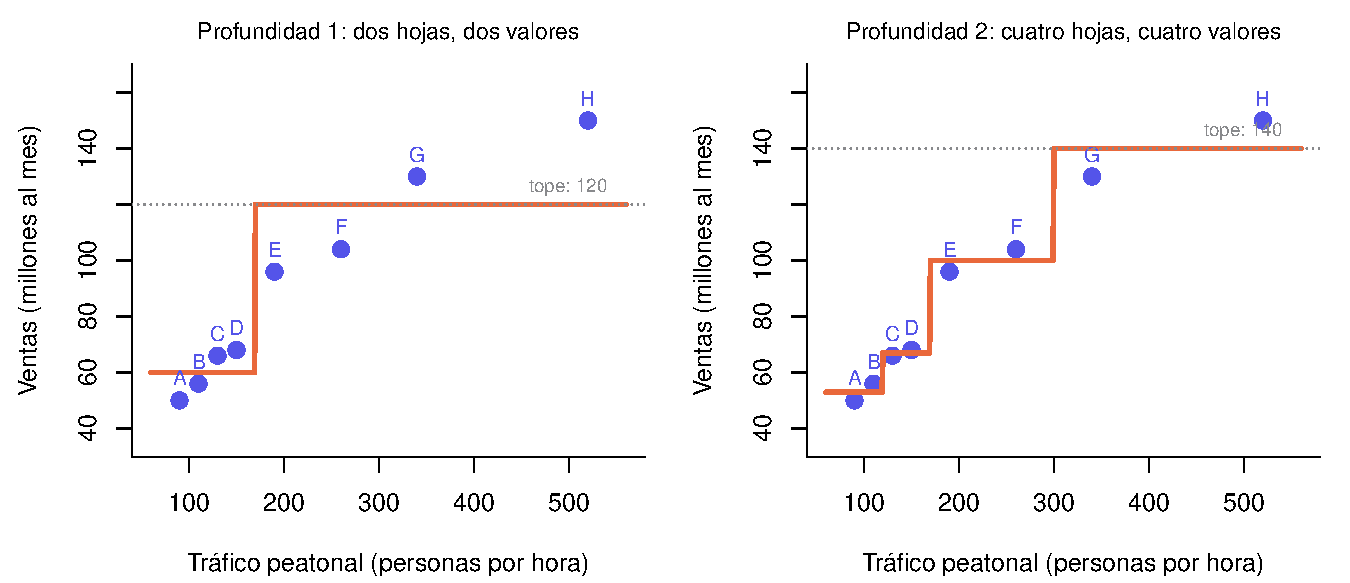
\includegraphics[width=0.76\textwidth]{figures/escalera_juguete.pdf}
\end{center}
\footnotesize
\begin{itemize}\itemsep2pt
  \item \textbf{k hojas, k valores.} Con un corte el árbol solo dice 60 o 120; con tres, 53, 67, 100 o 140. No hay rampa entre peldaños.
  \item \textbf{El tope.} H vende 150 y recibe 140. Un punto con 900 personas por hora también recibiría 140: el árbol no extrapola.
  \item \textbf{El error de construcción siempre baja:} MAE 30 (la mediana), 13.5 (un corte), 4.5 (tres cortes). Hasta cero si cada punto queda solo en su hoja: el memorizador.
\end{itemize}
\end{frame}

\begin{frame}{El promedio de una hoja a mano (III): la hoja real, n = 10}
\begin{center}
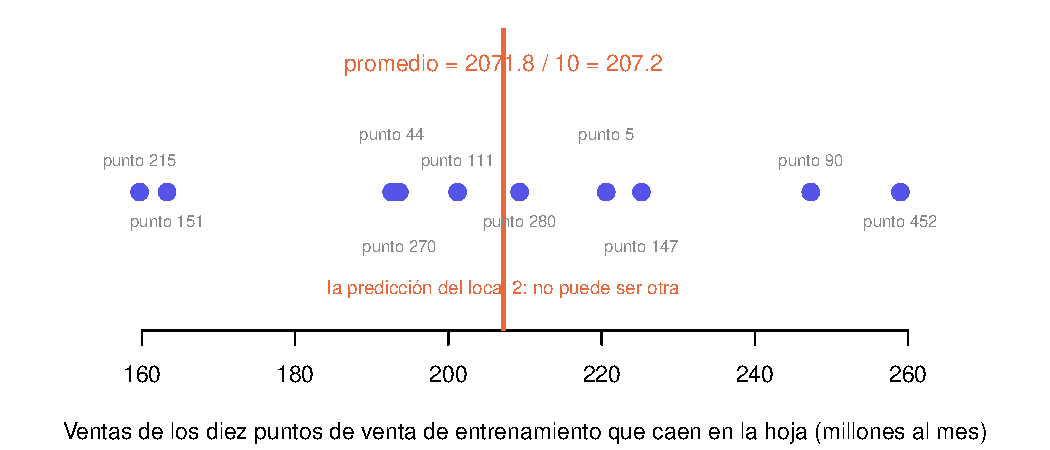
\includegraphics[width=0.7\textwidth]{figures/hoja_diez.pdf}
\end{center}
\begin{columns}[T]
\begin{column}{0.55\textwidth}
\footnotesize
La hoja más alta del árbol de profundidad 3: arriendo de 14.15 o más, tráfico de 318 o más y ticket promedio de 13.650 pesos o más. Diez puntos de venta de entrenamiento:
\smallskip

{\scriptsize 215: 159.7; 151: 163.3; 44: 192.6; 270: 193.6; 111: 201.2; 280: 209.3; 5: 220.6; 147: 225.2; 90: 247.3; 452: 259.0.}
\end{column}
\begin{column}{0.45\textwidth}
\footnotesize
Suma: 2.071.8. Promedio: $2071.8 / 10 = \mathbf{207.18}$.
\smallskip

Es la predicción del local 2 (arriendo 27, tráfico 760, ticket promedio 14.000): no puede ser otra, y no puede ser mayor. Es el tope del árbol.
\end{column}
\end{columns}
\end{frame}

\begin{frame}{Profundidad 3: ocho hojas, de 63.3 a 207.2}
\begin{center}
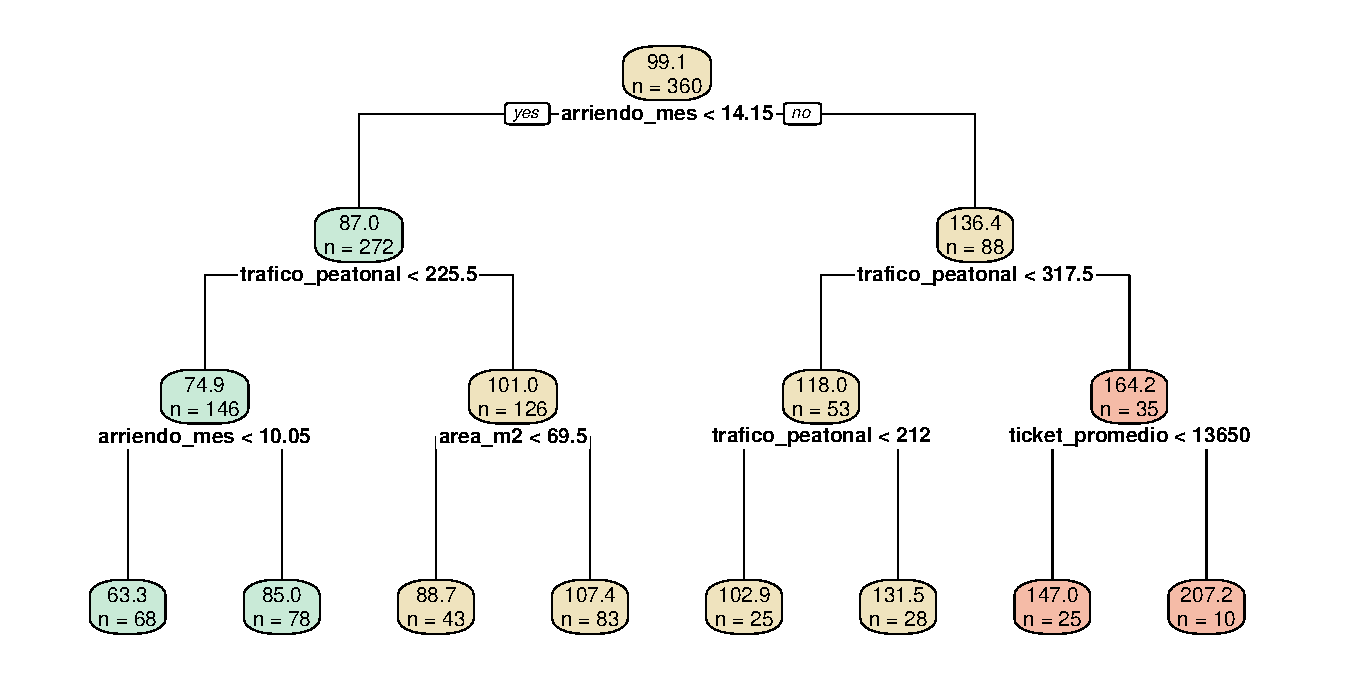
\includegraphics[width=0.95\textwidth]{figures/arbol_regresion_3.pdf}
\end{center}
\footnotesize
Es el árbol de referencia de las bandas. Añade el arriendo en 10.05, el área en 69.5, el tráfico en 212 y el ticket promedio en 13.650 pesos. Ocho valores posibles; el más alto, 207.2, con diez puntos de venta; el más bajo, 63.3, con 68. En validación: MAE \textbf{22.6} ($\pm$ 4.2), RMSE \textbf{32.2}.
\end{frame}

\begin{frame}{La tabla del líder en pesos (la versión de un equipo)}
\begin{columns}[T]
\begin{column}{0.55\textwidth}
{\footnotesize
\begin{tabular}{@{}lrr@{}}
\toprule
Predicción de ventas & MAE & RMSE \\
\midrule
Mediana del entrenamiento & 31.1 & 43.9 \\
Regla del sector: 8 $\times$ arriendo & 22.4 & 30.0 \\
Consultora A & 22.9 & 30.6 \\
Consultora B & 17.9 & 25.9 \\
\textbf{Árbol de profundidad 3} & \textbf{17.8} & \textbf{23.4} \\
\bottomrule
\end{tabular}}
\medskip

\small ``El árbol del equipo le gana a la consultora B (17.8 contra 17.9) y a la regla del sector por más de cuatro millones al mes. Recomendamos adoptarlo.''
\end{column}
\begin{column}{0.45\textwidth}
\parada{error sembrado}{¿Qué está mal en esta tabla? Dos minutos en parejas. Pista: ¿en qué puntos de venta se midió cada fila?}
\medskip
\footnotesize La fila del árbol es su MAE en los 360 puntos de venta con los que se construyó. Las otras cuatro, en los 120 de validación. En validación el árbol da \textbf{22.6}: empate con la regla. Es el bosque de Mullainathan y Spiess: 85 en entrenamiento, 45 en prueba.
\end{column}
\end{columns}
\end{frame}

\begin{frame}{La tabla del líder en pesos, en validación}
\begin{columns}[T]
\begin{column}{0.62\textwidth}
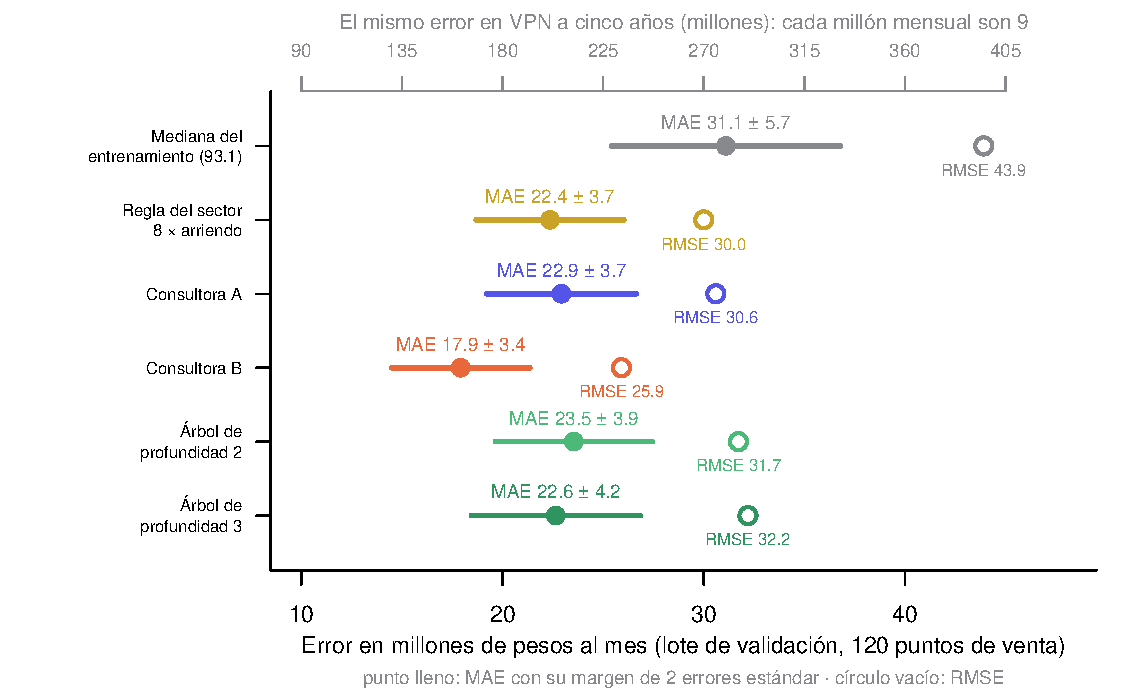
\includegraphics[width=\textwidth]{figures/lider_pesos.pdf}
\end{column}
\begin{column}{0.38\textwidth}
\footnotesize
Los 120 puntos de venta que ningún método vio. MAE con margen de dos errores estándar; RMSE al lado.
\medskip

\textbf{El árbol:} 22.6 $\pm$ 4.2 (prof. 3), 23.5 $\pm$ 3.9 (prof. 2).

\textbf{La regla:} 22.4 $\pm$ 3.7. \textbf{B:} 17.9 $\pm$ 3.4.
\medskip

En VPN a cinco años (9 por millón mensual): el error típico del árbol son \textbf{204 millones}; el de B, 161.
\medskip

La brecha MAE--RMSE (22.6 contra 32.2) anuncia errores grandes ocasionales: los vemos en dos láminas.
\end{column}
\end{columns}
\end{frame}

\begin{frame}{¿Le gana a la regla del sector? La comparación pareada}
\begin{center}
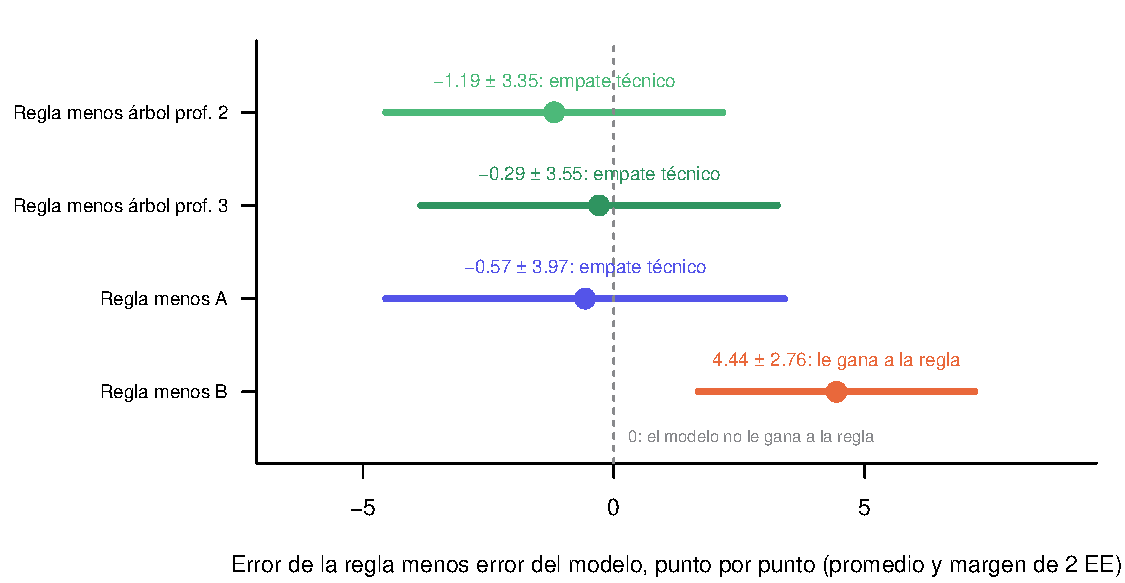
\includegraphics[width=0.6\textwidth]{figures/pareada_arbol.pdf}
\end{center}
\begin{columns}[T]
\begin{column}{0.55\textwidth}
\footnotesize Punto por punto: error de la regla menos error del modelo. Regla menos árbol de profundidad 3: $-0.29 \pm 3.55$; profundidad 2: $-1.19 \pm 3.35$. El margen cruza el cero: \textbf{empate técnico}, igual que A. Solo B le gana ($4.44 \pm 2.76$).
\end{column}
\begin{column}{0.45\textwidth}
\importa{Un árbol que empata con ``8 $\times$ arriendo'' no es inútil: dice lo que la gerencia de expansión ya sabe, con una banda medida. Pero no justifica una factura.}
\end{column}
\end{columns}
\end{frame}

\begin{frame}{El memorizador, en pesos}
\begin{columns}[T]
\begin{column}{0.55\textwidth}
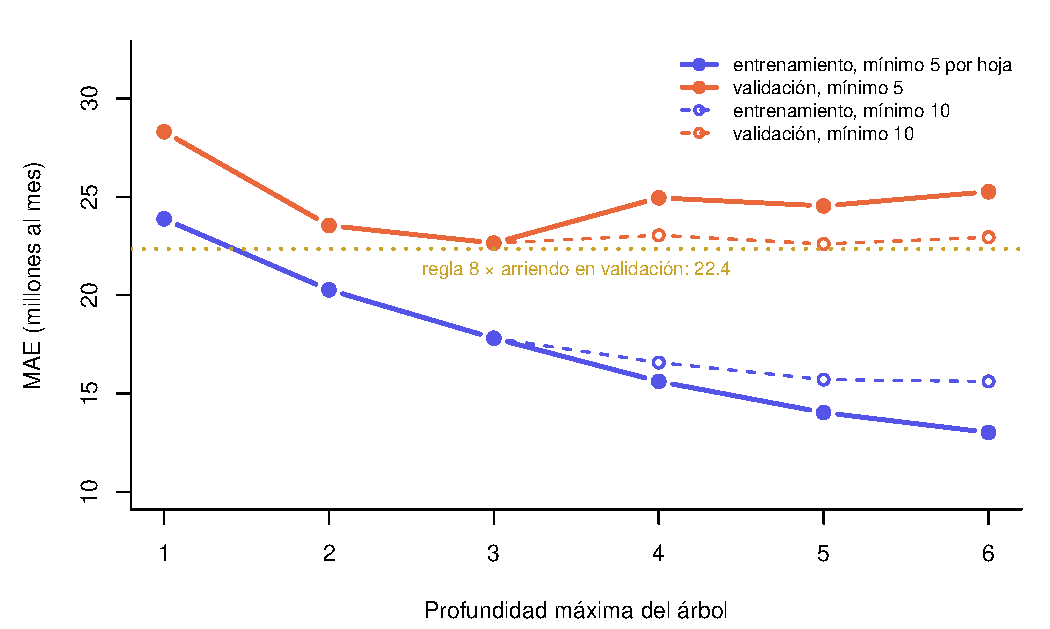
\includegraphics[width=\textwidth]{figures/memorizador_regresion.pdf}
\end{column}
\begin{column}{0.45\textwidth}
\small
\begin{itemize}\itemsep3pt
  \item Con mínimo 5 y profundidad 6, \textbf{33 hojas}: MAE 13.0 en entrenamiento y 25.3 en validación.
  \item La profundidad 3 (22.6) ya está en el fondo de la curva de validación; de ahí en adelante solo mejora la de entrenamiento.
  \item Ningún árbol le gana a la regla (22.4) por más que el ruido.
\end{itemize}
\parada{chat}{Un equipo reporta MAE 14 y RMSE 31. ¿Qué está pasando? Una línea.}
\end{column}
\end{columns}
\end{frame}

\begin{frame}{Dónde falla: los diez peores}
\begin{columns}[T]
\begin{column}{0.52\textwidth}
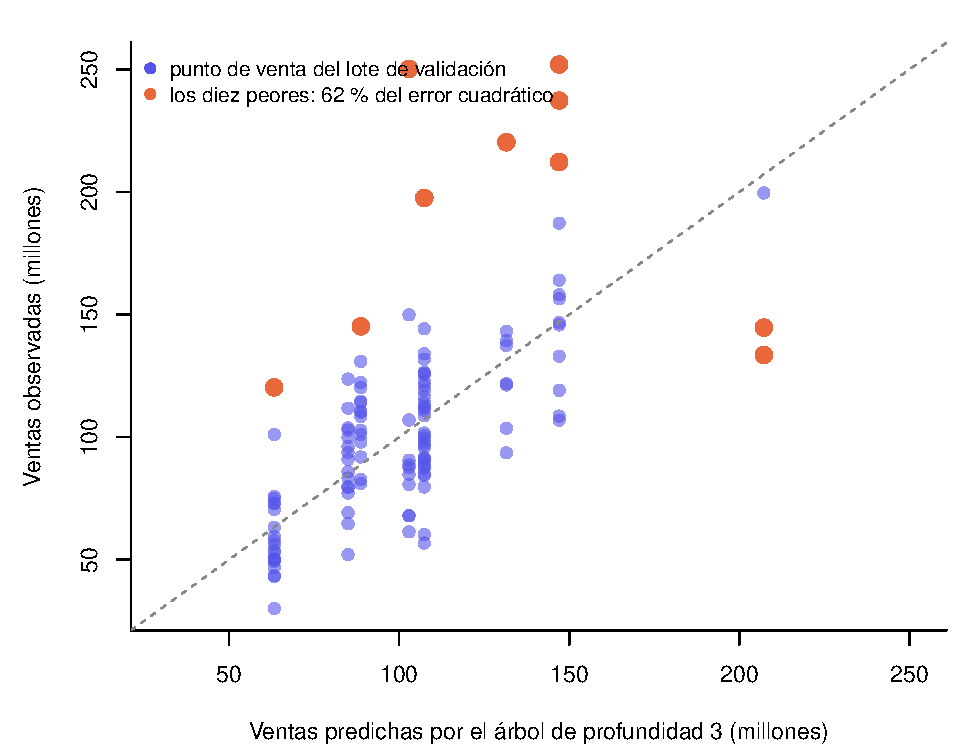
\includegraphics[width=\textwidth]{figures/arbol_regresion_residuos.pdf}
\end{column}
\begin{column}{0.48\textwidth}
\footnotesize
Diez puntos de venta de 120 concentran el \textbf{61.8\,\%} del error cuadrático. Ocho venden más de lo que el árbol dice; \textbf{seis pasan de 150 millones}; siete están en zona de oficinas. Los dos que el árbol sobreestima (366 y 36) caen en la hoja de 207.2.
\medskip

El punto 52 vende 250.2 y el árbol dice 102.9: un punto de venta estrella en una hoja de puntos típicos. Ninguna hoja pasa de 207.2.
\medskip

\importa{Tratamiento aparte: el modelo para la mayoría, una persona para los grandes. Sin los diez, el MAE baja a 17.1; esa cifra es un diagnóstico, no un desempeño. No se arregla con más profundidad.}
\end{column}
\end{columns}
\end{frame}

\begin{frame}{Las ventas base de los tres locales, con banda}
\begin{center}
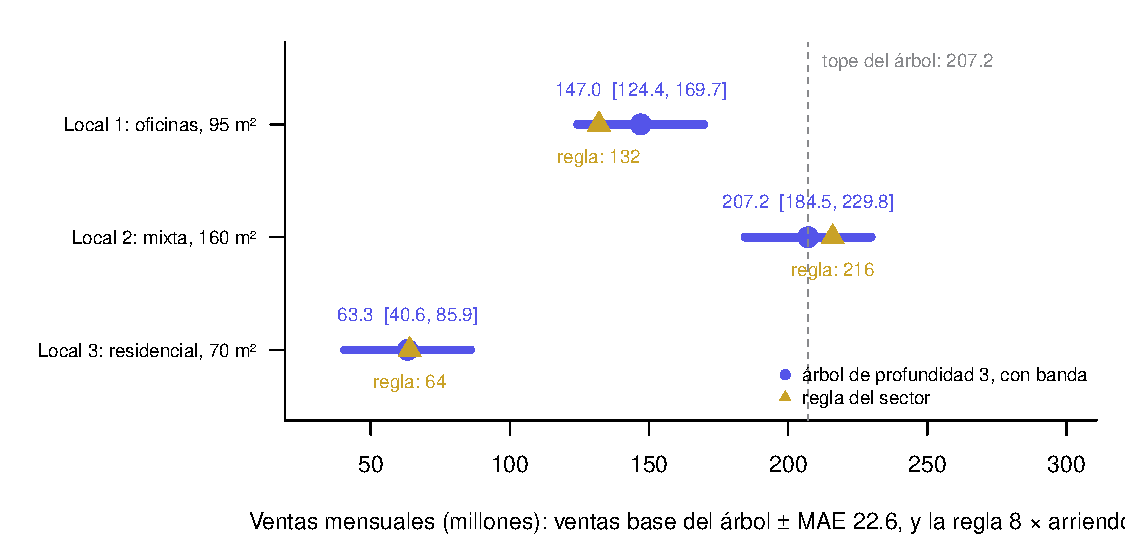
\includegraphics[width=0.7\textwidth]{figures/bandas_locales.pdf}
\end{center}
\begin{center}
{\scriptsize\setlength{\tabcolsep}{4pt}
\begin{tabular}{@{}lrlrl@{}}
\toprule
Local & Base & Banda ($\pm$ 22.6) & Regla 8 $\times$ & Nota de extrapolación \\
\midrule
Local 1 (oficinas) & 147.0 & [124.4, 169.7] & 132 & * ciudad \\
Local 2 (mixta) & 207.2 & [184.5, 229.8] & 216 & * ciudad; arriendo 27 $>$ 25; el tope \\
Local 3 (residencial) & 63.3 & [40.6, 85.9] & 64 & * ciudad \\
\bottomrule
\end{tabular}}
\end{center}
\footnotesize En VPN a cinco años ($\times$ 9): local 1, de 1.120 a 1.527; local 2, de 1.661 a 2.068; local 3, de 366 a 773. Son las \textbf{ventas base} de la semana 7, con la nota pegada. La regla cae dentro de la banda en los tres. Su rango de la encuesta: ¿cayó dentro de la banda del local 1?
\end{frame}

\begin{frame}{El giro: el arriendo del local 2 sube 30\,\%}
\begin{columns}[T]
\begin{column}{0.55\textwidth}
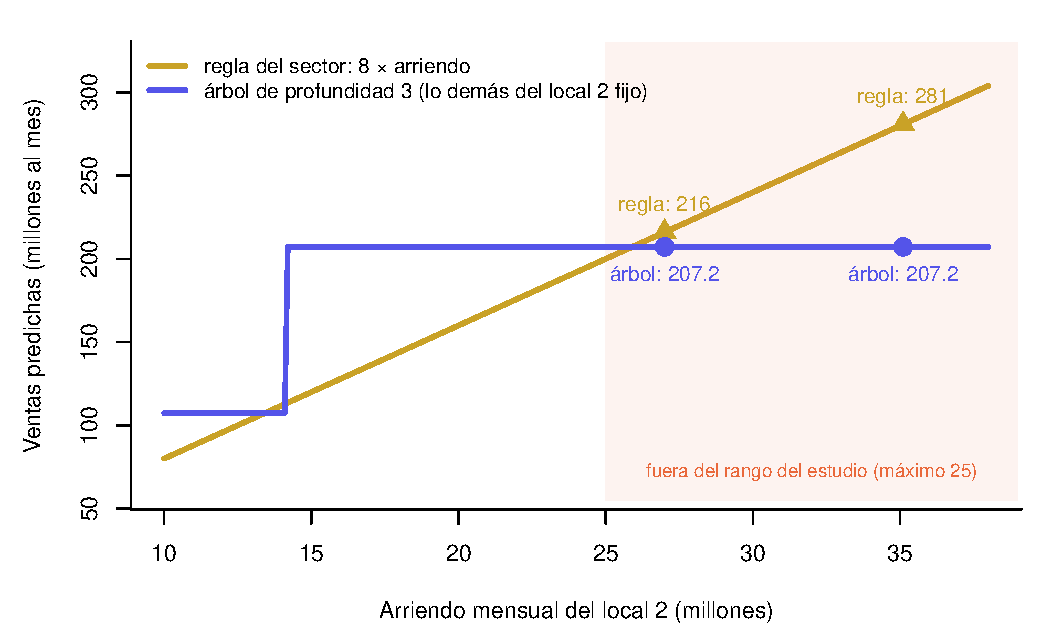
\includegraphics[width=\textwidth]{figures/giro_arriendo.pdf}
\end{column}
\begin{column}{0.45\textwidth}
\small
El arrendador del local 2 pide 35.1 millones en lugar de 27.
\medskip

\textbf{La regla:} de 216 pasa a \textbf{281}.

\textbf{El árbol:} sigue diciendo \textbf{207.2}. Misma hoja.
\medskip

\parada{el giro}{¿A cuál creerle, y por qué? Una línea por equipo.}
\footnotesize Ninguno mecánicamente. El árbol no extrapola: 27 ya estaba fuera del rango (máximo 25) y 35.1 más. La regla ignora todo lo demás: un arriendo más alto no aumenta las ventas. Lo que cambió es un costo, y eso entra al VPN, no a las ventas.
\end{column}
\end{columns}
\end{frame}

\begin{frame}{Lo que importa}
\importa{%
\begin{enumerate}\itemsep5pt
  \item \textbf{La hoja es un promedio y el árbol es una escalera.} k hojas, k valores; el más alto es el tope. No extrapola: fuera del rango, asterisco.
  \item \textbf{El error se reporta en pesos y fuera de muestra.} MAE 22.6 en validación (el 17.8 de entrenamiento no cuenta); en VPN, 204 millones. La brecha con el RMSE manda a mirar los diez peores.
  \item \textbf{Contra la vara, pareado.} El árbol empata con 8 $\times$ arriendo; solo el bosque le gana. Un empate con la regla no justifica una factura.
  \item \textbf{Lo que se entrega es una banda.} Ventas base $\pm$ error típico, con la nota de extrapolación pegada, en millones al mes y en VPN. Sin banda no es pronóstico; sin nota no cuenta.
\end{enumerate}}
\end{frame}

\seccion{El task y el cierre}
%% ====================================================== 3. PUENTE (65–70)
\begin{frame}{Task 6: la tabla del líder en pesos y las ventas base}
\small
\begin{columns}[T]
\begin{column}{0.55\textwidth}
\textbf{Qué se entrega} (una página, en equipo, antes de la sesión 7; se hace con la práctica 6, sin código):
\begin{itemize}\itemsep3pt
  \item la tabla del líder en pesos, contra el sobre (1.5);
  \item dónde falla el modelo y qué se haría ahí: los diez peores y el tratamiento aparte (1.0);
  \item las ventas base de los tres locales con su banda y su nota de extrapolación, con la regla 8 $\times$ al lado (1.5);
  \item la posición actualizada: registro de posición, toma 2, cinco líneas (0.5);
  \item el acta y la declaración (0.5).
\end{itemize}
\end{column}
\begin{column}{0.45\textwidth}
\begin{exampleblock}{En el cierre de la sesión 7}
Traen las bandas de los tres locales y su posición. Se discute ``¿le ganamos a la regla?'' y se comparan las bandas entre equipos.
\end{exampleblock}
\begin{alertblock}{Lo que no cuenta}
Un MAE de entrenamiento. Una banda sin nota de extrapolación. Una predicción por encima de la hoja más alta. Una fila que no coincida con el sobre sin explicar la diferencia.
\end{alertblock}
\end{column}
\end{columns}
\end{frame}

%% ====================================================== 4. CIERRE (70–90)
\begin{frame}{Cierre: el árbol del equipo (task 5)}
\begin{enumerate}\itemsep6pt
  \item \textbf{Una rama en voz alta} (8 minutos): cada equipo, al azar, traduce una rama de su árbol como se la diría a la junta, en un minuto. Sin ``nodo'', sin ``corte'', sin ``causa'', con p y n.
  \item \textbf{¿Aguantó la raíz?} (5 minutos): a mano alzada, ¿a quién le cambió la raíz al cambiar la semilla? Con la partición del curso es el tráfico en 164.5; con las semillas 101 y 202, 164.5 y 160.5. ¿Y el segundo nivel?
  \item \textbf{¿Qué sí se le dice a la junta?} (5 minutos): la primera pregunta y las hojas grandes; no el segundo nivel ni la hoja de 24 puntos de venta. Los locales de Barranquilla, siempre con asterisco.
  \item \textbf{Dudas} (2 minutos): la práctica 6 y la entrega del task 6.
\end{enumerate}
\end{frame}

\begin{frame}{Referencias}
\small
\begin{itemize}\itemsep4pt
  \item Mullainathan, S. y Spiess, J. (2017). Machine learning: an applied econometric approach. \emph{Journal of Economic Perspectives}, 31(2), 87--106. Tabla 1 y apéndice en línea (tabla B.1).
  \item Breiman, L., Friedman, J., Olshen, R. y Stone, C. (1984). \emph{Classification and Regression Trees}. Wadsworth.
  \item Breiman, L. (2001). Random forests. \emph{Machine Learning}, 45(1), 5--32.
  \item Kleinberg, J., Ludwig, J., Mullainathan, S. y Obermeyer, Z. (2015). Prediction policy problems. \emph{American Economic Review}, 105(5), 491--495.
  \item Sosa Escudero, W. (2019). \emph{Big data}. Siglo XXI. El capítulo sobre árboles y predicción.
\end{itemize}
\end{frame}

\end{document}
